\chapter{Ferramentas Computacionais}
\label{chap:ferramentas}

\lettrine{O}{} interesse no estudo de Desenvolvimento de Ontologias, Lógicas de Descrição e Revisão de Crenças, deve-se, em parte, às aplicações computacionais que tais áreas possuem. Neste capítulo, algumas delas serão abordadas.

\section{OWL}

O final da década de 1990 foi a época em que surgiu a ideia de Web Semântica. Esse conceito, já consolidado hoje, define uma parte da \textit{World Wide Web} onde é possível o trabalho cooperativo entre as máquinas e os seres humanos. Ele ocorre a partir dos significados que são dados aos conteúdos disponíveis na rede, para que haja compreensão por ambos os tipos de agentes \citep{ferramentasHerman}.

A fim de que alguma Linguagem de Representação fosse criada, a \href{https://www.w3.org}{W3C} (sigla para Consórcio para a \textit{World Wide Web}) fundou o "\textit{Web Ontology Working Group}", no início dos anos 2000  \citep{ferramentasGrupo}. 

Os primeiros rascunhos foram publicados em julho de 2002, e em fevereiro de 2004, a OWL (\textit{Web Ontology Language}) tornou-se o padrão recomendado pela W3C para o processamento de ontologias \citep{ferramentasReco}.

Em outubro de 2007, um novo grupo foi concebido para adicionar alguns recursos à linguagem. Dois anos depois, a W3C fez o lançamento da OWL 2, que seria compatível com editores e raciocinadores semânticos \citep{ferramentasOWLGrupo2}. Ela foi recomendada oficialmente pela W3C em dezembro de 2012 \citep{ferramentasOWLReco2}.

Abaixo estão algumas características das duas versões da OWL.

\subsection{OWL Web Ontology Language}

A primeira versão possui três sublinguagens \citep{ferramentasOWL1}. Cada uma possui suas particularidades:

\begin{itemize}
	\item \textit{Lite}: Sublinguagem mais simples, feita para hierarquias de classificação com restrições simples. Suporta restrições de cardinalidade simples (apenas 0 ou 1).  Foi demonstrado que OWL-Lite é equivalente a $ \mathcal{SHIF^{(D)}} $ \citep{ferramentasGrau}.
	\item DL: É equivalente a $ \mathcal{SHOIN^{(D)}} $. Oferece expressividade máxima evitando alguns problemas de decidibilidade. Inclui todos os construtores da OWL. Possui mais complexidade formal do que a sublinguagem \textit{Lite}.
	\item \textit{Full}: Versão mais completa, oferecendo expressividade máxima e a liberdade sintática do RDF, só que sem garantias computacionais. Nessa sublinguagem, pode acontecer de uma Classe ser tratada como uma coleção de indivíduos ou como um indivíduo, o que acarreta problemas de decidibilidade. Não corresponde a nenhuma lógica de descrição.
\end{itemize}

\subsection{OWL 2 Web Ontology Language}

A segunda versão também possui sublinguagens \citep{ferramentasOWL2}. Elas são:

\begin{itemize}
	\item EL: Corresponde à lógica $ \mathcal{EL} $++. Funciona bem para ontologias com muitas classes e/ou propriedades. Permite a existência de algoritmos de inferência polinimiais.
	\item QL: Baseada na lógica de descrição DL-\textit{Lite}, foi feita para aplicações em que o volume de instâncias é muito grande e que a consulta de dados é a tarefa mais realizada. Tais consultas podem até ser implementadas usando sistemas de bancos de dados convencionais.
	\item RL: Criada para ontologias que precisam de raciocínio escalável, ou seja, que são possivelmente grandes em número de instâncias, mas que precisam de uma sublinguagem que mantenha um bom poder expressivo. É baseada em uma lógica de descrição chamada DLP.
	\item DL: Assim como no lançamento anterior, oferece bastante expressividade, sem esbarrar em problemas de execução por causa da indecibilidade. Ela pode ser mapeada para a LD $ \mathcal{SROIQ^{(D)}} $. 
	\item \textit{Full}: Análoga à da primeira versão. Muito expressiva, porém, indecidível.
\end{itemize}

\section{\textit{Protégé}}

O \href{https://protege.stanford.edu}{\textit{Protégé}} é um editor semântico, compatível com a OWL 2. Ele foi desenvolvido pelo Centro de Pesquisa para Informática Biomédica da Universidade de Stanford, em colaboração com alguns programadores da Universidade de Manchester \footnote{\url{https://protege.stanford.edu/about.php}}. Sua primeira versão foi lançada em 1999, e a atual é de 2017. Seu logotipo está exibido na \autoref{img:Protege}.

Seguindo os princípios do \textit{Software} Livre, ele é um arcabouço gratuito e de código aberto, feito para a construção de sistemas inteligentes, com o uso ou não de uma interface gráfica.

Assim como o ambiente de desenvolvimento integrado Eclipse, o \textit{Protégé} é bastante flexível porque é possível desenvolver uma grande variedade de \textit{plug-ins} para serem acoplados a ele.

\begin{figure}[H]
	\centering
	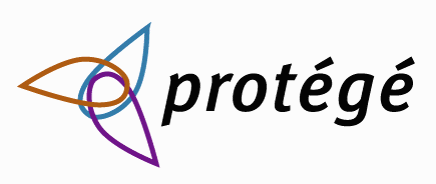
\includegraphics[width=0.5\textwidth]{Capitulos/Ferramentas/protege}
	\caption{O logotipo do \textit{Protégé}.}
	\label{img:Protege}
\end{figure}

Para exemplificar alguns recursos do \textit{Protégé}, será usada, como exemplo, parte da ontologia criada neste estudo:

\begin{itemize}
	\item Os conceitos: 
	\begin{itemize}
		\item \texttt{Musica} $ \equiv $ \texttt{Cancao} $ \sqcup $ \texttt{HinoNacional};
		\item \texttt{Pop} $ \sqsubseteq $ \texttt{Cancao};
		\item \texttt{EDM} $ \sqsubseteq $ \texttt{Cancao};
		\item \texttt{Pessoa} $ \equiv $ \texttt{Cantor} $ \sqcup $ \texttt{Compositor}.
	\end{itemize}
	\item As propriedades:
	\begin{itemize}
		\item \textbf{\texttt{canta}}, com domínio \texttt{Cantor} e contradomínio \texttt{Musica};
		\item \textbf{\texttt{cantadaPor}}, inversa da propriedade acima.
	\end{itemize}
	\item As instâncias e asserções:
	\begin{itemize}
		\item \texttt{MarinaAndTheDiamonds}, instância da classe \texttt{Cantor};
		\item \texttt{Primadonna}, instância da classe \texttt{Pop};
		\item \texttt{MarinaAndTheDiamonds \textbf{canta} Primadonna};
		\item \texttt{Froot}, instância da classe \texttt{Pop};
		\item \texttt{MarinaAndTheDiamonds \textbf{canta} Froot};
		\item \texttt{Disconnect}, instância da classe \texttt{EDM};
		\item \texttt{MarinaAndTheDiamonds \textbf{canta} Disconnect}.	
	\end{itemize}
\end{itemize}

No \textit{Protégé}, a ontologia fica como na \autoref{img:Representacao}.

\begin{figure}[H]
	\centering
	\begin{subfigure}{.3\textwidth}
		\centering
		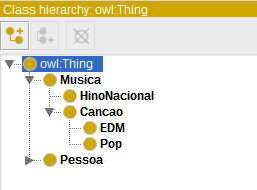
\includegraphics[width=0.95\linewidth]{Capitulos/Ferramentas/classes}
		\caption{A hierarquia das classes.}
	\end{subfigure}%
	\begin{subfigure}{.475\textwidth}
		\centering
		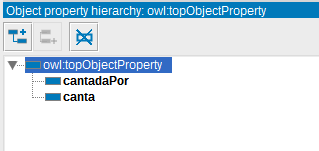
\includegraphics[width=0.95\linewidth]{Capitulos/Ferramentas/propriedades}
		\caption{As propriedades da ontologia.}
	\end{subfigure}
	\begin{subfigure}{.3\textwidth}
		\centering
		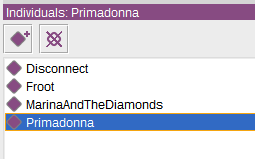
\includegraphics[width=0.95\linewidth]{Capitulos/Ferramentas/individuos}
		\caption{As instâncias definidas.}
	\end{subfigure}
	\caption{A representação da ontologia do \textit{Protégé}.}
	\label{img:Representacao}
\end{figure}
 
\subsection{Raciocinadores}

Um aspecto interessante sobre esse arcabouço é o uso de \textit{plug-ins} de raciocínio, como o HermiT \footnote{\url{http://www.hermit-reasoner.com/}}. A partir deles, é possível fazer inferências a partir dos axiomas lógicos que foram criados.

No fragmento da ontologia, temos que \texttt{MarinaAndTheDiamonds \textbf{canta} Primadonna}. É possível inferir que \texttt{Primadonna \textbf{cantadaPor} MarinaAndTheDiamonds}. O \textit{Protégé} consegue fazer isso com o auxílio do raciocinador, como exibido na \autoref{img:Raciocinador}.

\begin{figure}[H]
	\centering
	\begin{subfigure}{.5\textwidth}
		\centering
		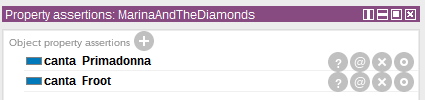
\includegraphics[width=0.9\linewidth]{Capitulos/Ferramentas/marinacanta}
		\caption{Músicas que \texttt{MarinaAndTheDiamonds} canta.}
	\end{subfigure}%
	\begin{subfigure}{.5\textwidth}
		\centering
		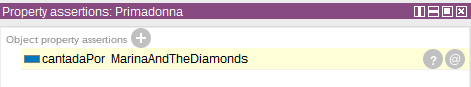
\includegraphics[width=0.95\linewidth]{Capitulos/Ferramentas/inferencia}
		\caption{Com o raciocinador, é mostrado quem canta Primadonna. O destaque indica inferência.}
	\end{subfigure}
	\caption{A asserção feita na construção da ontologia e a inferência feita.}
	\label{img:Raciocinador}
\end{figure}

\subsection{Buscas}

A partir de uma ontologia e de uma base de dados, é possível fazer buscas neste arcabouço, utilizando, entre várias linguagens de busca, o SPARQL.

SPARQL é um acrônimo recursivo para SPARQL \textit{Protocol and RDF Query Language}  \citep{ferramentasSPARQL}. Ele tem uma sintaxe que lembra a do SQL, e com seu uso, é possível tratar a ontologia como uma base de dados.  

Vale notar que as buscas funcionam apenas com a terminologia e as asserções gravadas no arquivo da ontologia. Para que as buscas funcionem sobre as inferências, é necessário exportá-las para um novo arquivo.

No exemplo utilizado, temos que \texttt{MarinaAndTheDiamonds} canta música de dois ritmos diferentes. Para descobrir quais são as músicas \texttt{Pop} que ela canta, pode-se rodar uma consulta, como na mostrada na \autoref{img:Consulta}.

\begin{figure}
	\centering
	\begin{subfigure}{.7\textwidth}
		\centering
		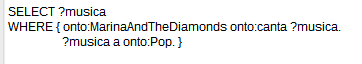
\includegraphics[width=0.95\linewidth]{Capitulos/Ferramentas/query}
		\caption{Fragmento da consulta para a pergunta. Note que o prefixo \texttt{onto} refere-se a definições dessa ontologia.}
	\end{subfigure}
	\begin{subfigure}{.7\textwidth}
		\centering
		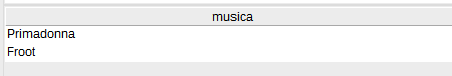
\includegraphics[width=0.95\linewidth]{Capitulos/Ferramentas/resultado}
		\caption{A consulta gera uma tabela com as músicas do ritmo \texttt{Pop} que \texttt{MarinaAndTheDiamonds} canta.}
	\end{subfigure}
	\caption{A consulta feita e seu resultado.}
	\label{img:Consulta}
\end{figure}